%!Mode::"TeX:UTF-8"
\documentclass[11pt]{article}
\usepackage{amsmath}
\usepackage{amssymb}
\usepackage{enumerate}
\usepackage{graphicx}
\usepackage[colorlinks,linkcolor=blue,anchorcolor=red,citecolor=green]{hyperref}
\usepackage{titlesec}
\usepackage{listings}
\usepackage{float}
\usepackage{paralist}
\usepackage{bm}
\usepackage{framed}
\usepackage{algorithm}
\usepackage[amsmath,thmmarks]{ntheorem}
%\usepackage[default]{sourcesanspro}
\usepackage[labelsep=quad]{caption}
\usepackage[top=2.54cm, bottom=2.54cm, left=2.54cm, right=2.54cm]{geometry}
\usepackage{fancyhdr}
 \pagestyle{fancy}
 \lhead{CS260 Homework3}
 \fancyfoot{}
 \rfoot{\thepage}
 
 \lstset{
  frame=tb,
  language=Java,
  aboveskip=3mm,
  belowskip=3mm,
  showstringspaces=false,
  columns=flexible,
  basicstyle={\small\ttfamily},
  numbers=none,
  numberstyle=\tiny\color{black},
  keywordstyle=\color{black},
  commentstyle=\color{black},
  stringstyle=\color{mauve},
  breaklines=true,
  breakatwhitespace=true
  tabsize=3
  escapeinside=``
}

\newtheorem{theorem}{Theorem}[section]
\newtheorem{definition}{Definition}[section]
\numberwithin{equation}{section}

\title{\textsc{CS260 Homework 3}}
\author{Yang Yang 804522285}
\date{Oct 5, 2015}


\begin{document}
       % generates the title
       \maketitle
       % insert the table of contents
       %\tableofcontents
	
%##########################################################
Collaborators:  Qian Li
\section{Question 1}
	After converting all training data into bag-of-words features vectors, from the matlab result we know that the most frequently 3 words are:
	\begin{center}
	\{(enron: $600$), (will: $451$), (please: $291$)\}
	\end{center}
\section{Question 2}
	For unregularized logistic regression:
	\begin{equation}
		w^{t+1} = w^t - \eta \sum_i \{\sigma({w^t}^Tx_i + b^t) - y_i\}x_i
	\end{equation}
	\begin{equation}
		b^{t+1} = b^t - \eta \sum_i \{\sigma({w^t}^Tx_i + b^t) - y_i\}
	\end{equation}
		\\[2ex]
	For regularized logistic regression:
	\begin{equation}
		w_j^{t+1} = w_j^t - \eta\{ \sum_i \{\sigma({w^t}^Tx_i + b^t) - y_i\}x_{i,j} + 2\lambda w_j^t\}
	\end{equation}
	\begin{equation}
		b^{t+1} = b^t - \eta \sum_i \{\sigma({w^t}^Tx_i + b^t) - y_i\}
	\end{equation}

\section{Question 3}
	\subsection{Part a}
	
	\begin{figure} [H]
    	\centering 
    	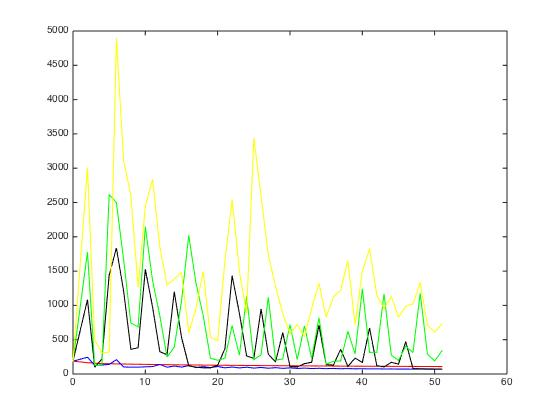
\includegraphics[width=4in]{Q3(a)} 
    	\caption{cross-entropy function value with respect to the number of steps for Ionosphere(yellow represent step size = $0.5$; green represent step size = $0.1$; black represent step size = $0.05$; blue represent step size = $0.01$; red represent step size = $0.001$)} 
    	\label{fig:side:a} 
	\end{figure}
	
	\begin{figure} [H]
    	\centering 
    	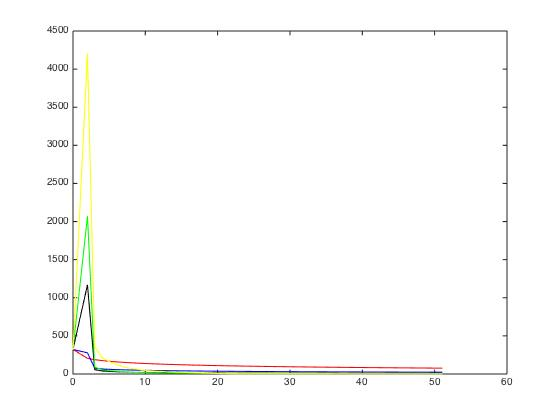
\includegraphics[width=4in]{Q3(a)_spam} 
    	\caption{cross-entropy function value with respect to the number of steps for EmailSpam(yellow represent step size = $0.5$; green represent step size = $0.1$; black represent step size = $0.05$; blue represent step size = $0.01$; red represent step size = $0.001$)} 
    	\label{fig:side:a} 
	\end{figure}
	
	\subsection{Part b}
	
	\begin{tabular}{cccccc}
	\hline
	$L2 norm (without regularization)$& 0.001& 0.01& 0.05& 0.1& 0.5\\
	\hline
	Ionosphere& 1.4855& 4.6573& 18.4769& 38.5544& 185.9563\\
	\hline	
	EmailSpam& 2.5806& 7.8507& 27.4529& 53.4542& 264.7956\\	
	\hline
	\end{tabular}
	
\section{Question 4}
	\subsection{Part a}
	\begin{figure} [H]
    	\centering 
    	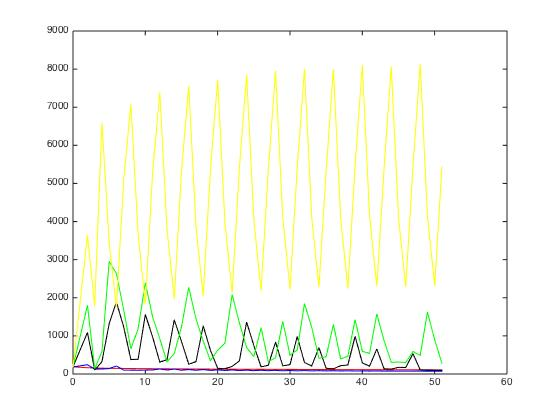
\includegraphics[width=4in]{4(a)1} 
    	\caption{cross-entropy function with regularization value with respect to the number of steps for Ionosphere(yellow represent step size = $0.5$; green represent step size = $0.1$; black represent step size = $0.05$; blue represent step size = $0.01$; red represent step size = $0.001$)} 
    	\label{fig:side:a} 
	\end{figure}

	
	\begin{figure} [H]
    	\centering 
    	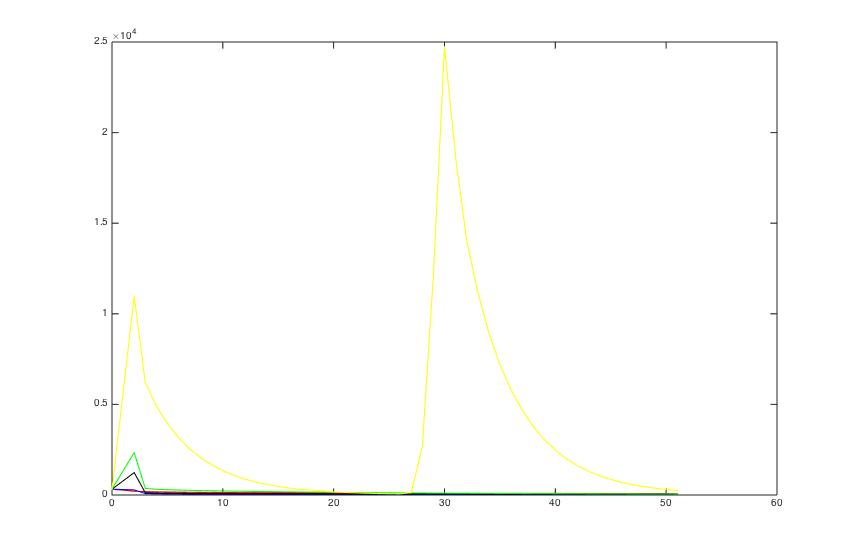
\includegraphics[width=7in]{4(a)_2} 
    	\caption{cross-entropy function with regularization value with respect to the number of steps for EmailSpam(yellow represent step size = $0.5$; green represent step size = $0.1$; black represent step size = $0.05$; blue represent step size = $0.01$; red represent step size = $0.001$)} 
    	\label{fig:side:a} 
	\end{figure}
	
	\subsection{Part b}
	
	\begin{tabular}{|c|c|c|c|c|c|c|c|c|c|}
	\hline
	$L2 norm (with regularization)$& 0& 0.05& 0.1& 0.15& 0.2& 0.25& 0.3& 0.35\\
	\hline
	Ionosphere& 4.6573& 4.5766& 4.4990& 4.4242& 4.3521& 4.2829& 4.2164& 4.1526\\
	\hline	
	EmailSpam& 7.8507& 7.6080& 7.3784& 7.1611& 6.9557& 6.7614& 6.5777& 6.4041\\	
	\hline
	$L2 norm (with regularization)$& 0.4& 0.45& 0.5\\
	\hline
	Ionosphere& 4.0908& 4.0300& 3.9712\\
	\hline
	EmailSpam& 6.2400& 6.0848& 5.9382\\
	\hline
	\end{tabular}
	
	\subsection{Part c}
	Entropy function with respect to regularization  cofficient for Ionosphere are shown below:

	\begin{figure} [H] 
	\centering
    	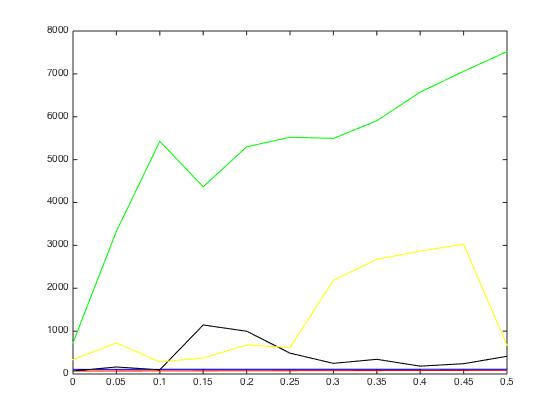
\includegraphics[width=4in]{Q5_2} 
    	\caption{entropy function with respect to regularization cofficient for Ionosphere(blue line: represent step size $=  0.001$, red line represent step size$ = 0.01$, black line represent step size $= 0.05$, yellow line represent step size$ = 0.1$, green line represent step size$ = 0.5$)} 
    	\label{fig:side:a} 
	\end{figure}
	
	Entropy function with respect to regularization  cofficient for EmailSpam are shown below:
	
	\begin{figure} [H] 
	\centering
    	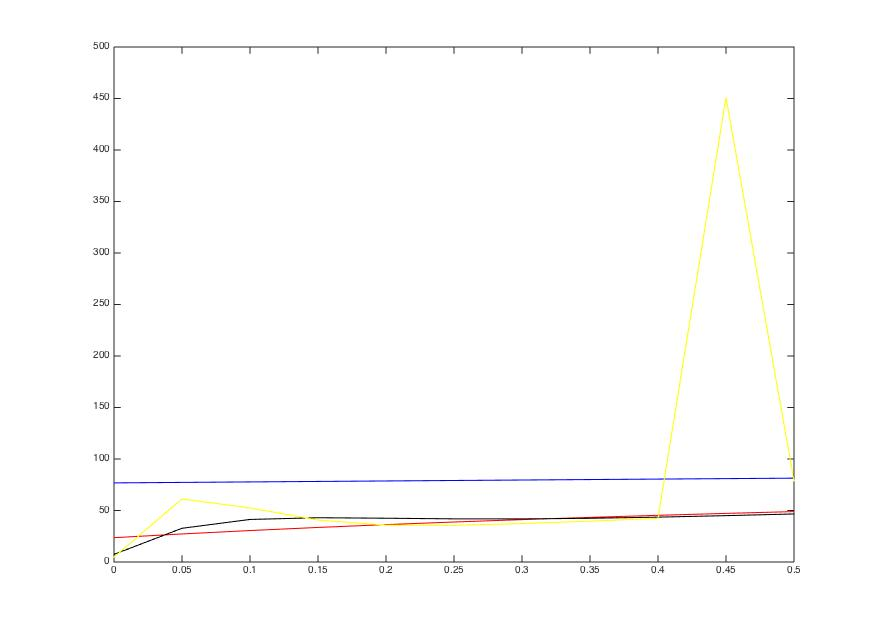
\includegraphics[width=4in]{Q5_1} 
    	\caption{entropy function with respect to regularization cofficient for EmailSpam(blue line: represent step size $=  0.001$, red line represent step size$ = 0.01$, black line represent step size $= 0.05$, yellow line represent step size$ = 0.1$)} 
    	\label{fig:side:a} 
	\end{figure}
	
	In the Figure 5, I did not include the situation when step size equals to 0.5. This is because the error function in this situation will be too large. You can see this situation in the below Figure 6.
	
	\begin{figure} [H] 
	\centering
    	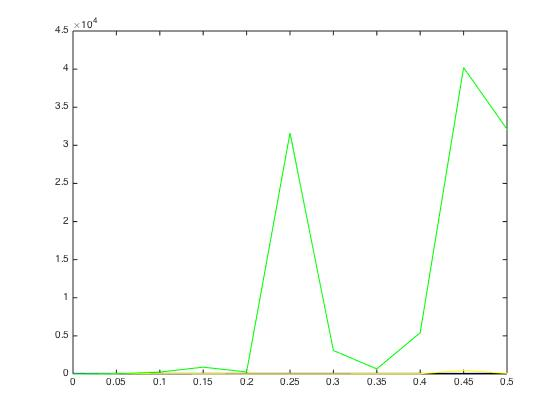
\includegraphics[width=4in]{Q5_3} 
    	\caption{entropy function with respect to regularization cofficient for EmailSpam(blue line: represent step size $=  0.001$, red line represent step size$ = 0.01$, black line represent step size $= 0.05$, yellow line represent step size$ = 0.1$, green line represent step size$ = 0.5$)} 
    	\label{fig:side:a} 
	\end{figure}

\section{Question 5}
	For unregularized logistic regression:
	\begin{equation}
	\bigtriangledown{\varepsilon_t(w)} =  \sum_i \{\sigma({w}^Tx_i + b) - y_i\}x_i
	\end{equation}
	
	\begin{equation}
	\mathbb{H}(w) = \sum_i{\{x_ix_i^T\sigma(\omega^Tx_i+b)[1 - \sigma(\omega^Tx_i+b)]\}}
	\end{equation}
	
	\begin{equation}
	\bigtriangledown{\varepsilon_t(b)} =  \sum_i \{\sigma({w}^Tx_i + b) - y_i\}
	\end{equation}
	
	\begin{equation}
	\mathbb{H}(b) = \sum_i{\{\sigma(\omega^Tx_i+b)[1 - \sigma(\omega^Tx_i+b)]\}}
	\end{equation}
	
	Thus, we can get the update function as follows
	
	\begin{equation}
	\begin{split}
	w^{t+1} &= w^t - \mathbb{H}^{-1}\bigtriangledown{\varepsilon_t} \\
	&= w^t - \{\sum_i{\{x_ix_i^T\sigma({w^t}^Tx_i+b^t)[1 - \sigma({w^t}^Tx_i+b^t)]\}}\}^{-1}\{\sum_i \{\sigma({w^t}^Tx_i + b^t) - y_i\}x_i\}
	\end{split}
	\end{equation}
	
	\begin{equation}
	\begin{split}
	b^{t+1} &= b^t - \mathbb{H}^{-1}\bigtriangledown{\varepsilon_t} \\
	&=b^t-\{\sum_i{\{\sigma({w^t}^Tx_i+b)[1 - \sigma({w^t}^Tx_i+b)]\}}\}^{-1}\{ \sum_i \{\sigma({w^t}^Tx_i + b^t) - y_i\}\}
	\end{split}
	\end{equation}
	\\[2ex]
	For regularized logistic regression:
	\begin{equation}
	 \frac{\partial}{\partial{w_j}}(\varepsilon_t(w_j))  =  \sum_i \{\sigma({w}^Tx_i + b) - y_i\}x_{i,j} + 2\lambda w_j
	\end{equation}
	
	\begin{equation}
	\frac{\partial^2}{\partial{ww^T}}(\varepsilon_t(w_j))  = \sum_i{\{x_ix_i^T\sigma(\omega^Tx_i+b)[1 - \sigma(\omega^Tx_i+b)]\}} + 2\lambda E
	\end{equation}
	
	\begin{equation}
	\bigtriangledown{\varepsilon_t(b)} =  \sum_i \{\sigma({w}^Tx_i + b) - y_i\}
	\end{equation}
	
	\begin{equation}
	\mathbb{H}(b) = \sum_i{\{\sigma(\omega^Tx_i+b)[1 - \sigma(\omega^Tx_i+b)]\}}
	\end{equation}
	Thus, we can get the update function as follows
\begin{equation}
	\begin{split}
	w_j^{t+1} &= w_j^t - \mathbb{H}^{-1}\bigtriangledown{\varepsilon_t} \\
	&= w_j^t - \{ \sum_i{\{x_{i,j}x_{i,j}^T\sigma({w^t}^Tx_i+b^t)[1 - \sigma({w^t}^Tx_i+b^t)]\}} + 2\lambda E\}^{-1}\{\sum_i \{\sigma({w^t}^Tx_i + b^t) - y_i\}x_{i,j} + 2\lambda w_j^t\}
	\end{split}
	\end{equation}


	\begin{equation}
	\begin{split}
	b^{t+1} &= b^t - \mathbb{H}^{-1}\bigtriangledown{\varepsilon_t} \\
	&=b^t-\{\sum_i{\{\sigma(\omega^Tx_i+b)[1 - \sigma(\omega^Tx_i+b)]\}}\}^{-1}\{ \sum_i \{\sigma({w}^Tx_i + b) - y_i\}\}
	\end{split}
	\end{equation}
	
\section{Question 6}
	\subsection{Part a}
	\begin{figure} [H]
    	\centering 
    	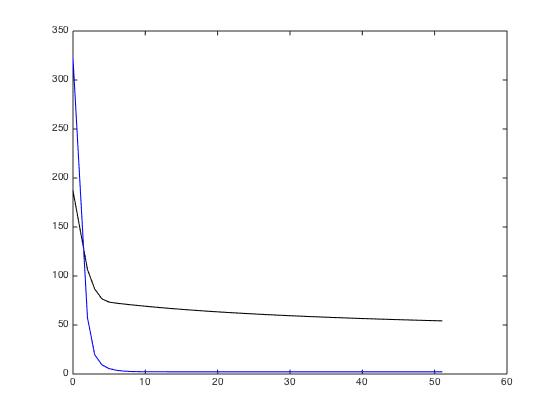
\includegraphics[width=4in]{Q6(a)} 
    	\caption{cross-entropy function with regularization value with respect to the number of steps for Ionosphere(black represent ionosphere and blue represent EmailSpam)} 
    	\label{fig:side:a} 
	\end{figure}
	\subsection{b}
	For ionosphere, the L2 norm for $w$ is 11.6866 
	
	For EmailSpam, the L2 norm for $w$ is 603.3280
	\subsection{c}
	For ionosphere, the error function value is 40.0021
	
	For EmailSpam, the error function value is 3697.6
\section{Question 7}
	\subsection{a}
	For $\lambda = 0$, it's the same as question 6.
	
	For $\lambda = 0.05$, it's the same as question 6.
	\begin{figure} [H]
    	\centering 
    	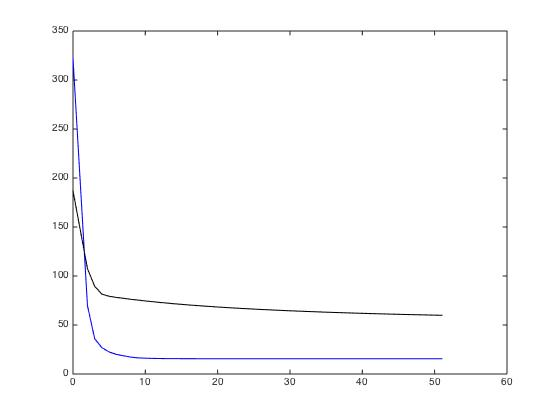
\includegraphics[width=4in]{Q7005} 
    	\caption{When $\lambda = 0.05$, cross-entropy function with regularization value with respect to the number of steps (black represent ionosphere and blue represent EmailSpam)} 
    	\label{fig:side:a} 
	\end{figure}

	For $\lambda = 0.1$, it's the same as question 6.
	\begin{figure} [H]
    	\centering 
    	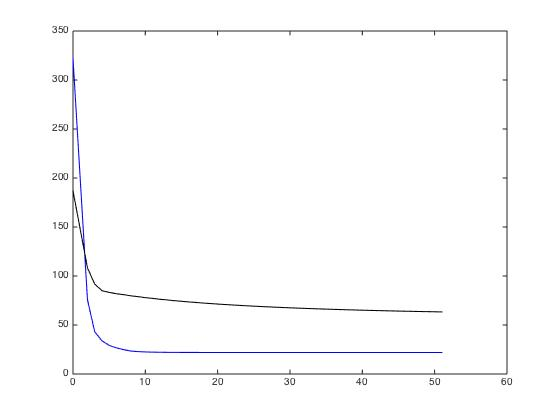
\includegraphics[width=4in]{Q701} 
    	\caption{When $\lambda = 0.1$, cross-entropy function with regularization value with respect to the number of steps (black represent ionosphere and blue represent EmailSpam)} 
    	\label{fig:side:a} 
	\end{figure}

	For $\lambda = 0.15$, it's the same as question 6.
	\begin{figure} [H]
    	\centering 
    	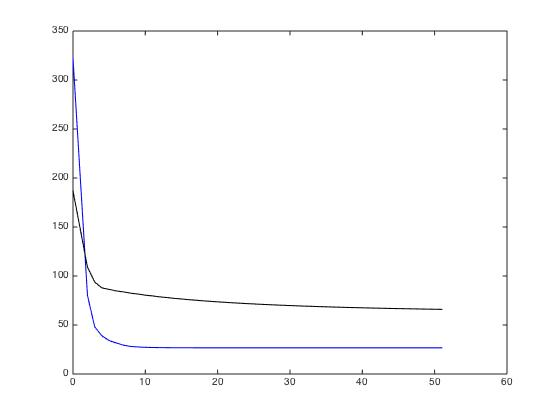
\includegraphics[width=4in]{Q7015} 
    	\caption{When $\lambda = 0.15$, cross-entropy function with regularization value with respect to the number of steps (black represent ionosphere and blue represent EmailSpam)} 
    	\label{fig:side:a} 
	\end{figure}

	For $\lambda = 0.2$, it's the same as question 6.
	\begin{figure} [H]
    	\centering 
    	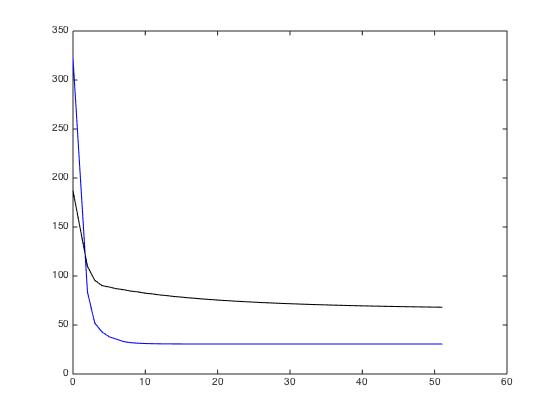
\includegraphics[width=4in]{Q702} 
    	\caption{When $\lambda = 0.2$, cross-entropy function with regularization value with respect to the number of steps (black represent ionosphere and blue represent EmailSpam)} 
    	\label{fig:side:a} 
	\end{figure}
	
	For $\lambda = 0.25$, it's the same as question 6.
	\begin{figure} [H]
    	\centering 
    	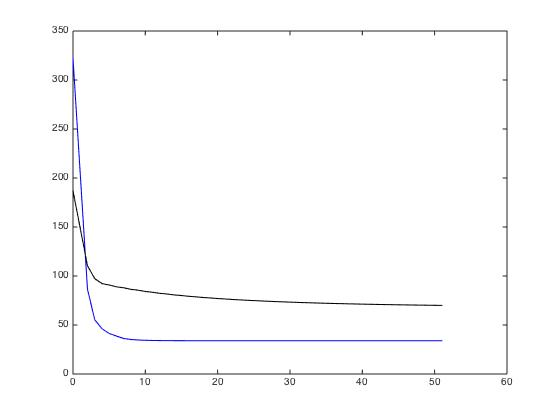
\includegraphics[width=4in]{Q7025} 
    	\caption{When $\lambda = 0.25$, cross-entropy function with regularization value with respect to the number of steps (black represent ionosphere and blue represent EmailSpam)} 
    	\label{fig:side:a} 
	\end{figure}
	
	For $\lambda = 0.3$, it's the same as question 6.
	\begin{figure} [H]
    	\centering 
    	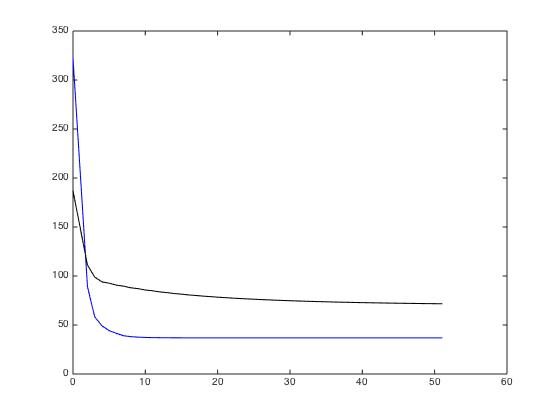
\includegraphics[width=4in]{Q703} 
    	\caption{When $\lambda = 0.3$, cross-entropy function with regularization value with respect to the number of steps (black represent ionosphere and blue represent EmailSpam)} 
    	\label{fig:side:a} 
	\end{figure}
	
	For $\lambda = 0.35$, it's the same as question 6.
	\begin{figure} [H]
    	\centering 
    	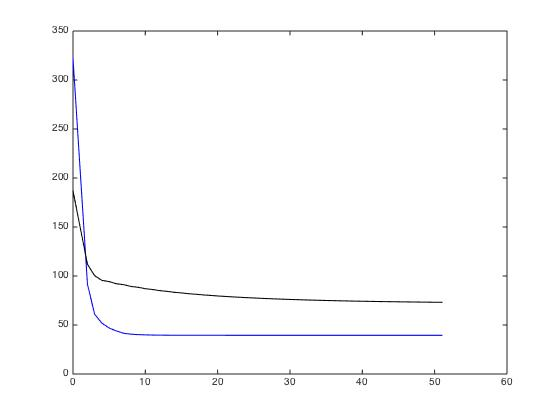
\includegraphics[width=4in]{Q7035} 
    	\caption{When $\lambda = 0.35$, cross-entropy function with regularization value with respect to the number of steps (black represent ionosphere and blue represent EmailSpam)} 
    	\label{fig:side:a} 
	\end{figure}
	
	For $\lambda = 0.4$, it's the same as question 6.
	\begin{figure} [H]
    	\centering 
    	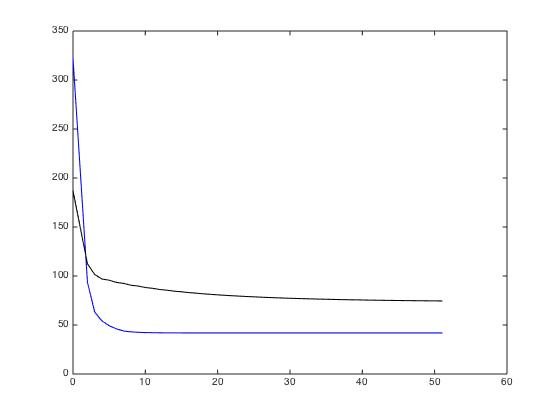
\includegraphics[width=4in]{Q704} 
    	\caption{When $\lambda = 0.4$, cross-entropy function with regularization value with respect to the number of steps (black represent ionosphere and blue represent EmailSpam)} 
    	\label{fig:side:a} 
	\end{figure}
	
	For $\lambda = 0.45$, it's the same as question 6.
	\begin{figure} [H]
    	\centering 
    	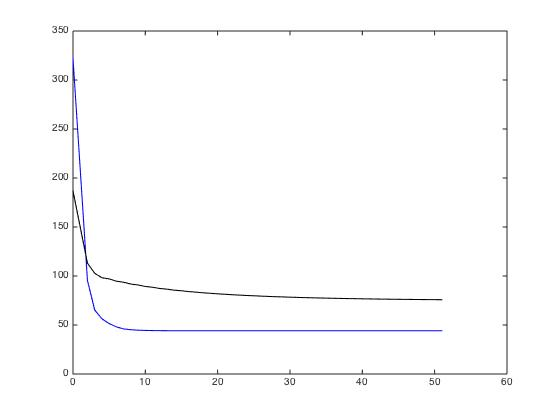
\includegraphics[width=4in]{Q7045} 
    	\caption{When $\lambda = 0.45$, cross-entropy function with regularization value with respect to the number of steps (black represent ionosphere and blue represent EmailSpam)} 
    	\label{fig:side:a} 
	\end{figure}

	For $\lambda = 0.5$, it's the same as question 6.
	\begin{figure} [H]
    	\centering 
    	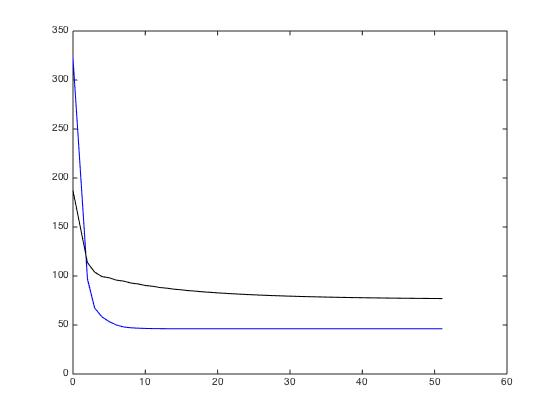
\includegraphics[width=4in]{Q705} 
    	\caption{When $\lambda = 0.5$, cross-entropy function with regularization value with respect to the number of steps (black represent ionosphere and blue represent EmailSpam)} 
    	\label{fig:side:a} 
	\end{figure}


	For $\lambda = 0.5$, it's the same as question 6.
	\begin{figure} [H]
    	\centering 
    	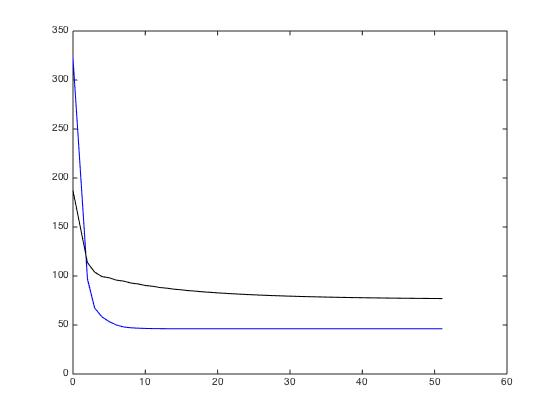
\includegraphics[width=4in]{Q705} 
    	\caption{When $\lambda = 0.5$, cross-entropy function with regularization value with respect to 	the number of steps(black represent ionosphere and blue represent EmailSpam)} 
    	\label{fig:side:a} 
	\end{figure}

	To compare the result, I put all Ionosphere plots in one picture and all EmailSpam plots in one picture. The pictures are shown below:
	
	\begin{figure} [H] 
    	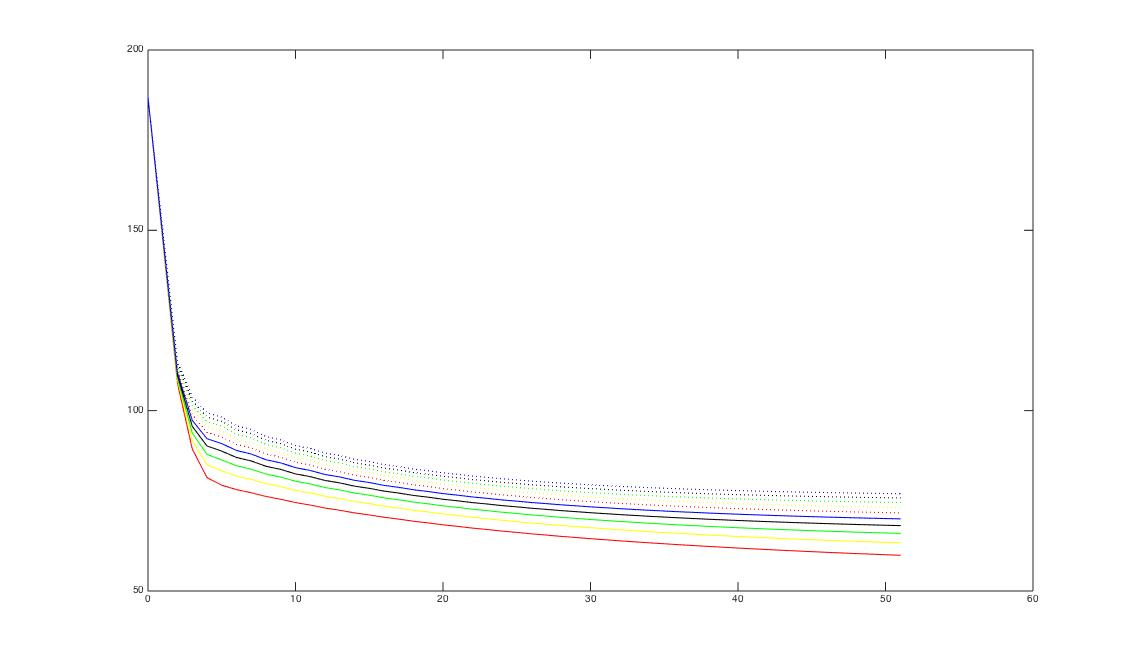
\includegraphics[width=6in]{Q7} 
    	\caption{ cross-entropy function  value with respect to the number of steps for Ionosphere(red solidline: $\lambda = 0.05$, yellow solidline: $\lambda = 0.1$, green solidline:$\lambda = 0.15$, black solidline: $\lambda = 0.2$, blue solidline: $\lambda = 0.25$,red dashed line: $\lambda = 0.3$, yellow dashed line: $\lambda = 0.35$, green dashed line:$\lambda = 0.4$, black dashed line: $\lambda = 0.45$, blue dashed line: $\lambda = 0.5$, )} 
    	\label{fig:side:a} 
	\end{figure}
	
	\begin{figure} [H] 
    	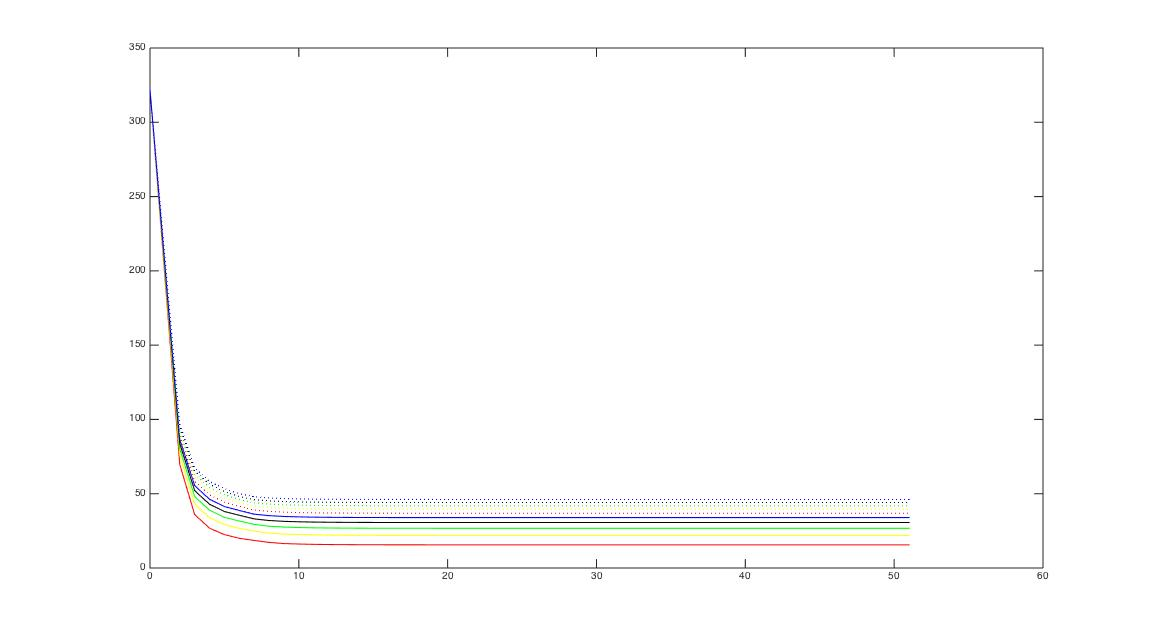
\includegraphics[width=6in]{Q7_spam} 
    	\caption{ cross-entropy function  value with respect to the number of steps for EmailSpam(red solidline: $\lambda = 0.05$, yellow solidline: $\lambda = 0.1$, green solidline:$\lambda = 0.15$, black solidline: $\lambda = 0.2$, blue solidline: $\lambda = 0.25$,red dashed line: $\lambda = 0.3$, yellow dashed line: $\lambda = 0.35$, green dashed line:$\lambda = 0.4$, black dashed line: $\lambda = 0.45$, blue dashed line: $\lambda = 0.5$, )} 
    	\label{fig:side:a} 
	\end{figure}
	
	\subsection{Part b}
	\begin{tabular}{|c|c|c|c|c|c|c|c|c|c|}
	\hline
	$L2 norm (with regularization)$& 0& 0.05& 0.1& 0.15& 0.2& 0.25& 0.3& 0.35\\
	\hline
	Ionosphere& 11.68& 8.57& 7.29& 6.54& 6.03& 5.65& 5.36& 5.11\\
	\hline	
	EmailSpam& 603.3& 12.46& 10.36& 9.22& 8.4543& 7.88& 7.4395& 7.07\\	
	\hline
	$L2 norm (with regularization)$& 0.4& 0.45& 0.5\\
	\hline
	Ionosphere& 4.91& 4.74& 4.58\\
	\hline
	EmailSpam& 6.76& 6.50& 6.27\\
	\hline
	\end{tabular}

	
	\subsection{Part c}
	\begin{tabular}{|c|c|c|c|c|c|c|c|c|c|}
	\hline
	error Function & 0& 0.05& 0.1& 0.15& 0.2& 0.25& 0.3& 0.35\\
	\hline
	Ionosphere& 40.0& 32.80& 31.10& 30.97& 31.37& 31.9247& 32.5178& 33.10\\
	\hline	
	EmailSpam& 3697.6& 122.35& 116.12& 113.92& 113.0654& 112.8121& 112.88& 113.15\\	
	\hline
	error Function & 0.4& 0.45& 0.5\\
	\hline
	Ionosphere& 33.67& 34.21& 34.72\\
	\hline
	EmailSpam& 113.54& 114.0& 114.51\\
	\hline
	\end{tabular}

\section{Question 8}
	From Figure 1 to Figure 4, we can see that if step size is too small, the convergence will be slow. But if step size is too large, the result will be unstable. It may now show convergence.
	
	From the table in 4.2, we can see that magnitude of w will be smaller with the increase of $\lambda$.
	
	If the step size is too large, the error function will increase steeply with the increase of step size. And it will increase very slowly with the increase of $\lambda$
	
\section{Question 9}
	When using gradient descent, you should choose the step size very carefully. But using newton's method could not consider this problem and it can convergence at the second iteration. However, the calculation of newton's method is more complex than gradient descent. It will take much longer time to compute newton's method than gradient descent.


\end{document}